\begin{titlepage}
    \begin{tikzpicture}[remember picture,overlay]
        \node[inner sep=0pt,anchor=south west] at (current page.south west) {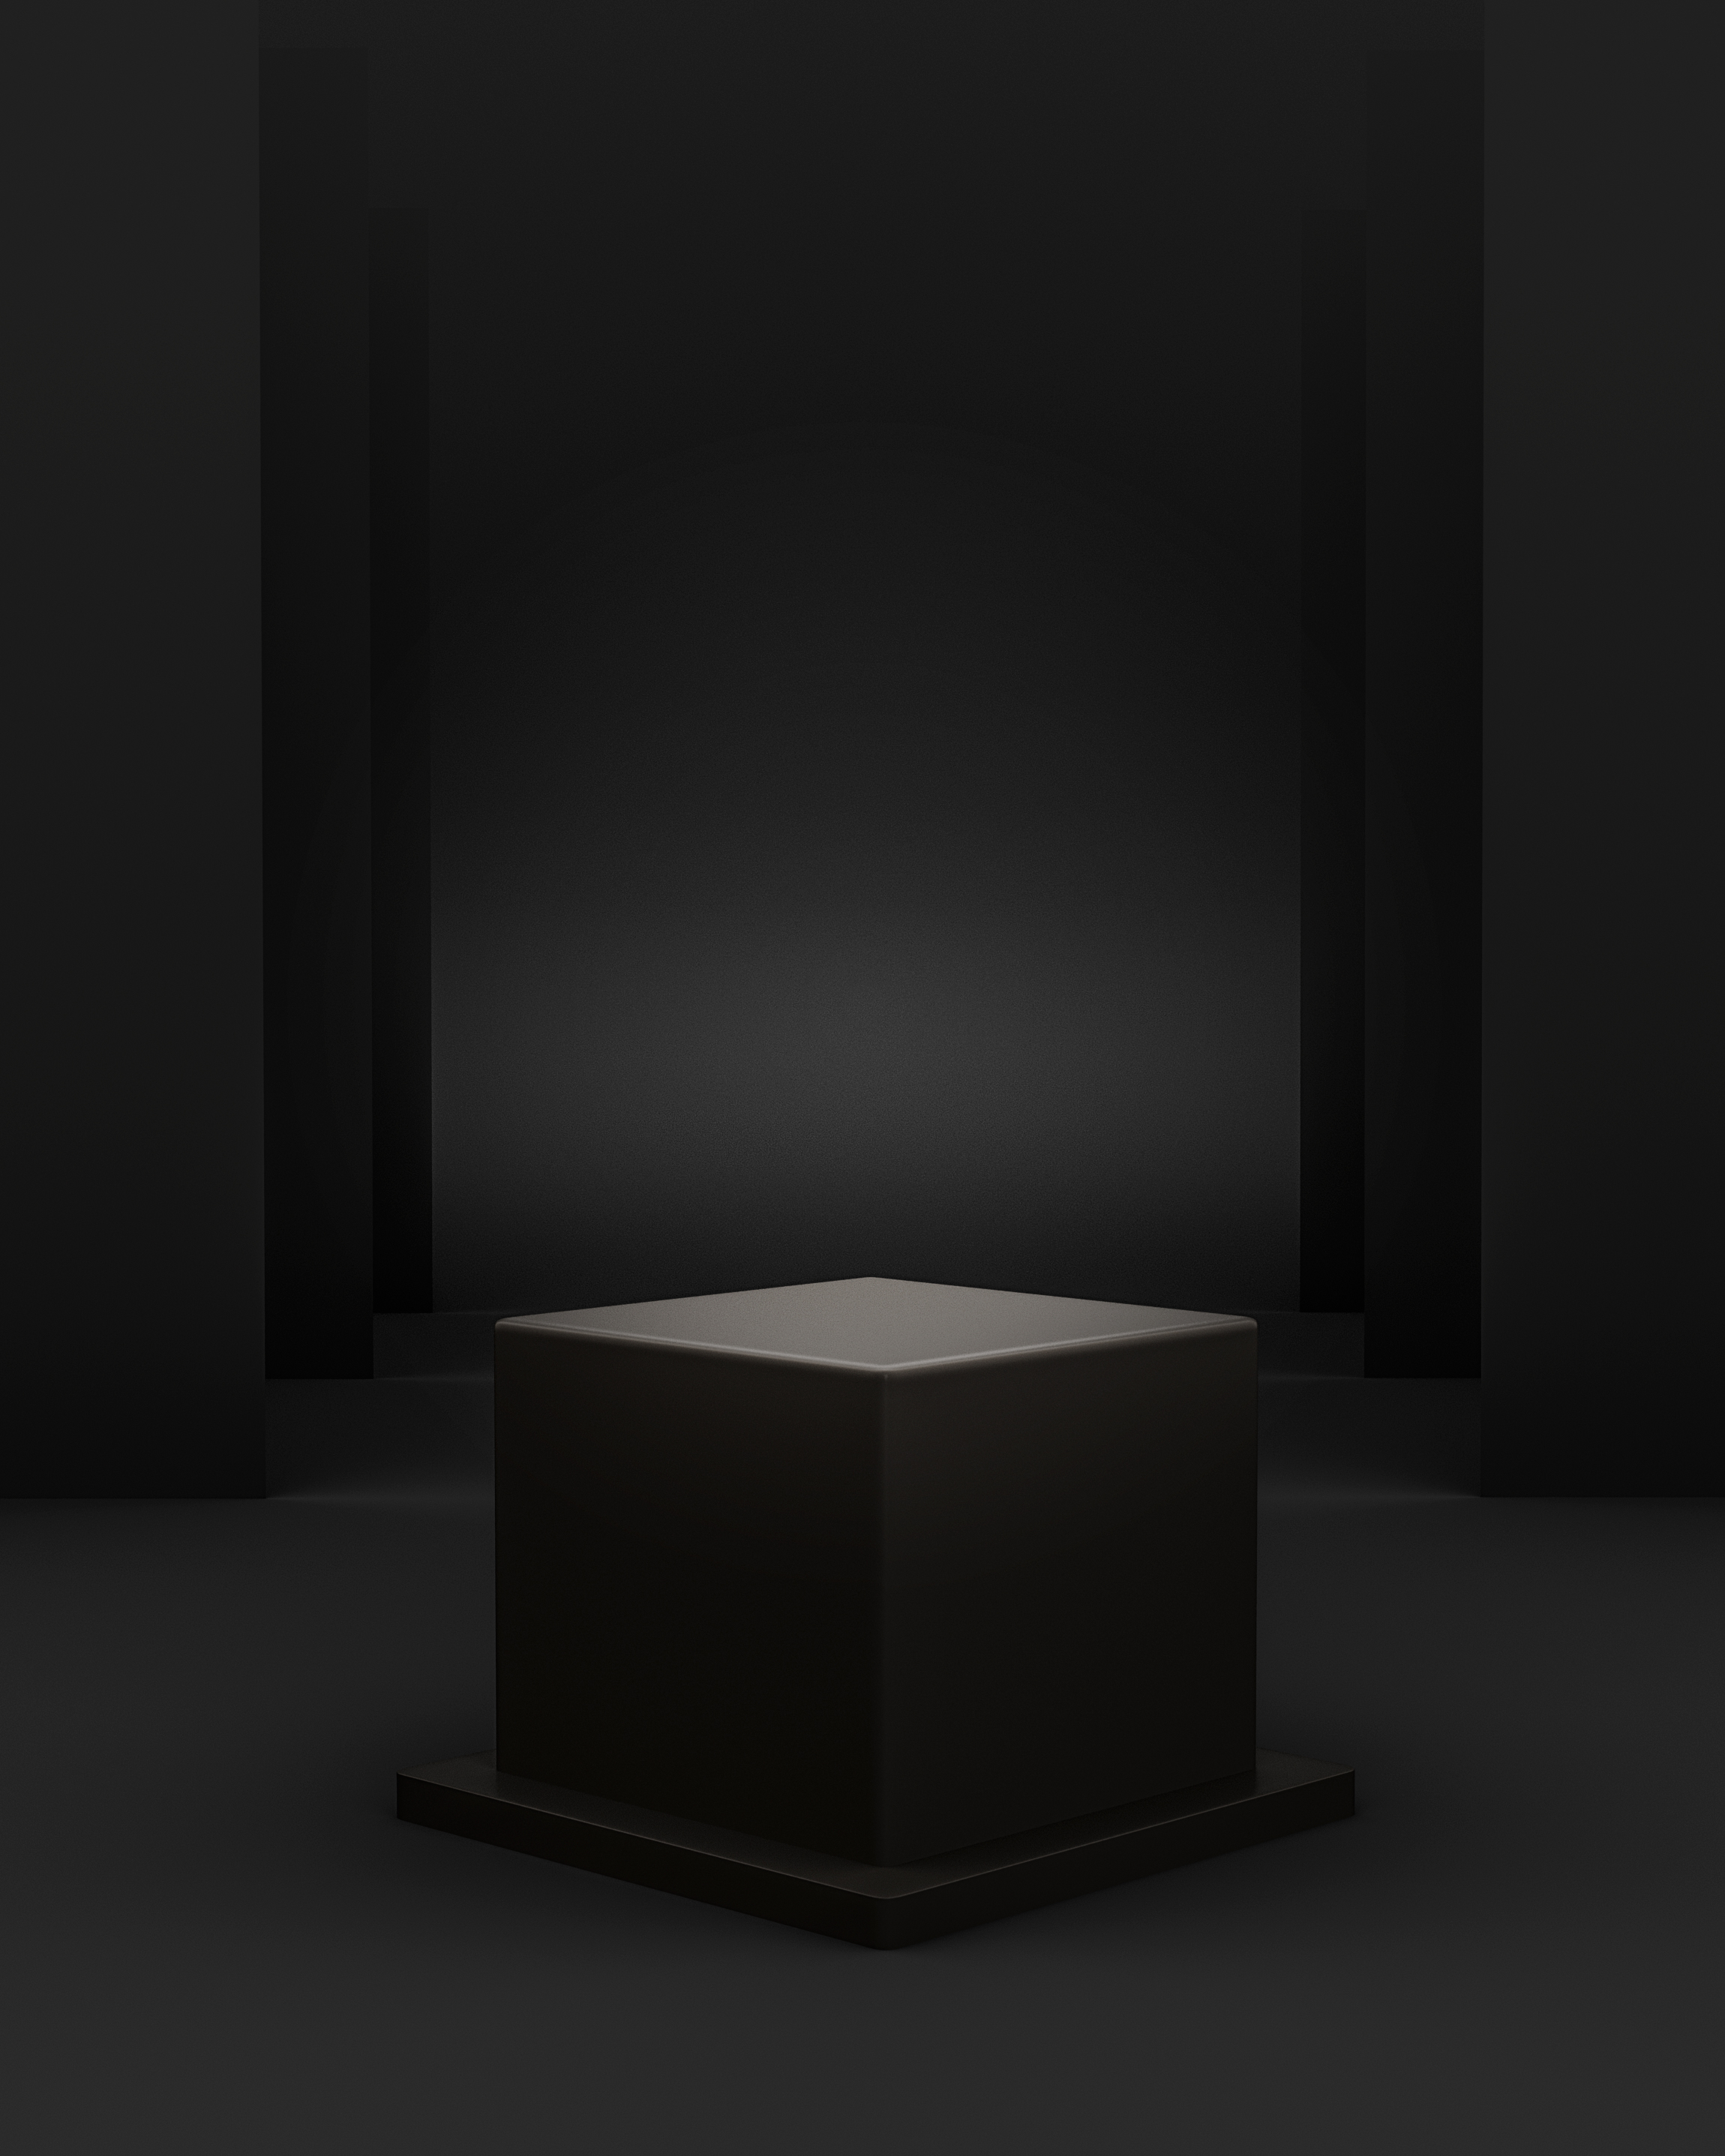
\includegraphics[width=\paperwidth,height=\paperheight]{preamble/titlepage.jpeg}};
    \end{tikzpicture}
    
    \begin{center}
    	\color{white} % Set the text color to white
        \vspace*{5cm} % Adjust this as needed to position your title vertically
		\Large \textbf{104295}        \\
		\vspace{0.5cm}
        \Huge \textbf{חשבון אינפיניטסימלי 3}
        \vspace{0.5cm}
        \rule{\linewidth}{0.5mm}
        \vspace{1cm}
        \Large רשימות תרגול - חורף תשפ"ד \\
        \vspace{0.5cm}
        \normalsize הפקולטה למתמטיקה בטכניון
        \vspace{0.5cm}
        \rule{\linewidth}{0.5mm}
        \vfill
        \normalsize נכתב על ידי רן קירי
    \end{center}
\end{titlepage}